% !TEX program = xelatex
% 编译：latexmk -xelatex main.tex（自动运行 BibTeX）
\documentclass[UTF8,fontset=none,zihao=-4,linespread=1,a4paper]{ctexart}
\usepackage{sysu-proposal}

% ===== 封面信息：只需修改右侧内容 =====
\renewcommand{\ProposalTitle}{填写论文题目}
\renewcommand{\ProposalName}{填写姓名}
\renewcommand{\ProposalStudentID}{填写学号}
\renewcommand{\ProposalMajor}{填写专业}
\renewcommand{\ProposalDirection}{填写研究方向}
\renewcommand{\ProposalSupervisor}{填写指导教师}
\renewcommand{\ProposalDegree}{博/硕士}
% 原 Word 封面标注为“二零二三版”，保留模版版本而非编译年份。
\renewcommand{\ProposalVersion}{二零二三版}

\begin{document}
\MakeProposalCover

\begin{proposalabstract}
在此填写开题报告摘要。
\end{proposalabstract}

% 原 Word 未要求目录。需要时取消下面两行的注释。
% \tableofcontents
% \clearpage

\section{课题来源/选题背景、研究的目的和意义}
\subsection{课题来源/选题背景}
在此填写课题来源和选题背景。

\subsection{研究目的及意义}
在此填写研究目的及意义。

\section{国内外研究现状及分析}
\subsection{国外研究现状}
在此填写国外研究现状。文献引用示例：英文期刊文献\cite{jaworski2009}。

\subsection{国内研究现状}
在此填写国内研究现状。文献引用示例：中文期刊文献\cite{liang1997}。

\subsection{国内外文献综述的简析}
在此填写国内外文献综述的简析。图书文献和译著引用示例\cite{tang1999,hosney1989}。

\section{研究内容、实施方案及研究计划}
\subsection{主要研究内容}
在此填写主要研究内容。图\ref{fig:workflow}给出了研究流程的示例。

% ===== 图示例：替换 figures/example-flow.pdf 即可使用自己的图片 =====
\begin{figure}[htbp]
  \centering
  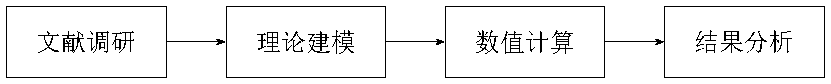
\includegraphics[width=0.85\linewidth]{figures/example-flow.pdf}
  \caption{研究流程示例}
  \label{fig:workflow}
\end{figure}

\subsection{实施方案/研究方法、实施计划及其可行性论证}
在此填写实施方案、研究方法、实施计划及其可行性论证。

% ===== 款标题和项示例；不需要时可删除 =====
\Needspace{132bp}
\begin{samepage}
\subsubsection{理论模型示例}
以一维简谐振子为例，运动方程见式\eqref{eq:oscillator}。

% ===== 公式示例：自动按一级章节编号为 (3-1) =====
\begin{equation}
  m\frac{\mathrm{d}^{2}x}{\mathrm{d}t^{2}}+kx=0.
  \label{eq:oscillator}
\end{equation}

\begin{proposalitems}
  \item 建立模型\quad 明确研究对象、基本假设与边界条件。
  \item 验证结果\quad 比较理论分析与数值计算结果。
\end{proposalitems}
\end{samepage}

\section{研究条件及进展}
在此填写研究条件及已完成的研究工作。会议论文、学位论文与电子文献的引用示例\cite{zhang1996,jin1998,wen1999}。

\section{论文目标及计划}
\subsection{学位论文预期创新点}
在此填写学位论文预期创新点。

\subsection{学位论文预期目标}
在此填写学位论文预期目标。

\subsection{学位论文进度安排}
在此填写学位论文进度安排，示例见表\ref{tab:schedule}。

% ===== 表示例：表题在表格上方，居中 =====
\begin{table}[htbp]
  \centering
  \caption{学位论文进度安排示例}
  \label{tab:schedule}
  \begin{tabularx}{0.9\linewidth}{c X X}
    \toprule
    阶段 & 主要工作 & 预期成果 \\
    \midrule
    第一阶段 & 文献调研与问题凝练 & 完成研究方案 \\
    第二阶段 & 理论分析与数值计算 & 获得主要研究结果 \\
    第三阶段 & 结果整理与论文撰写 & 完成学位论文 \\
    \bottomrule
  \end{tabularx}
\end{table}

\section{预计研究过程中可能遇到的困难、问题，以及解决的途径}
在此填写预计遇到的困难、问题及解决途径。

% 自动生成第 7 节“主要参考文献”，不要再手写 \section。
% 文献按正文首次引用顺序排列。只输出已引用的条目。
\bibliographystyle{sysu-proposal}
\bibliography{references}
\end{document}
